\documentclass[letterpaper,english, 12pt]{article}
\usepackage[T1]{fontenc}
\usepackage{lmodern}
\usepackage{graphicx}
\usepackage{textcomp}
\usepackage{float}
\usepackage{amsmath}
\usepackage{verbatim}
\usepackage{minipage}
\usepackage[lofdepth,lotdepth]{subfig}

\begin{titlepage}
                \begin{center}
                        \vspace*{1cm}

                        \LARGE{\textbf{WINDRONE: Gesture-Controlled Flight of an AR Drone}}

                        \vspace{0.5cm}
                        \large{Tae-Min Kim, Nikhil Shenoy, Felix Yeung, Shu Xu}
                        \vspace{1.5cm}

                        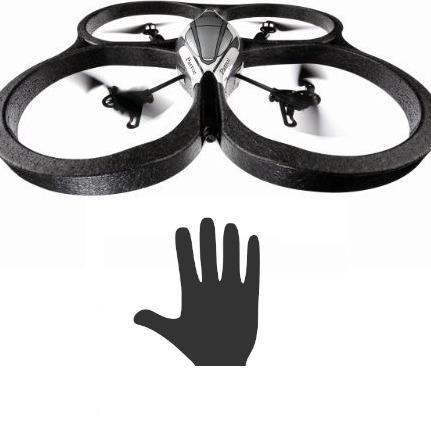
\includegraphics[height=8cm, width=100mm]{pics/titlepic.jpg}

			\vspace{2cm}
                        \small{Advisers: Roy Yates and Ivan Seskar}  \\
                        Course: 14:332:492 Special Problems/Independent Study \\
                        Rutgers University Department of Electrical and Computer Engineering \\
                        5/23/2014

                \end{center}
\end{titlepage}


\begin{document}

\newpage

\section*{Abstract}
	In this study, we create a new interface to decrease the difficulty of controlling the Parrot AR Drone, a radio controlled flying quadcopter helicopter. Rather than using the default iOS/Android application, we enable a simpler, more intuitive, and more natural control module: hand gestures. Taking advantage of new technology called the Leap Motion Controller \textemdash a device which is able to sense the user's hands and fingers \textemdash we create a system for users to send instructions directly to the AR Drone based on the positioning of their hand. Although originally intended for users to be able to more easily control AR Drones, this study may also be used to further study human-computer interaction as well.

\section*{Introduction to Flight Dynamics}
\begin{itemize}
		\item Yaw: left or right rotation with relation to the normal axis of the center of mass  of the object. Example: \\
		\begin{figure}[H]
			\centering
			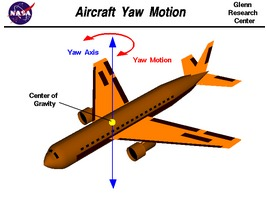
\includegraphics[height=6cm, width=80mm]{pics/yaw1.jpg} 
			\caption{Example of Yaw}
		\end{figure}
		\item Pitch: rotation along the lateral axis of the object. In the example of a plane, the lateral axis is measured from wingtip to wingtip. Example:
		\begin{figure}[H]
			\centering
			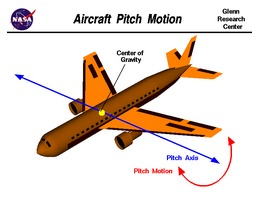
\includegraphics[height=6cm, width=80mm]{pics/pitch1.jpg} 
			\caption{Example of Pitch}
		\end{figure}
		\item Roll: rotation along the longitudinal axis of the object.In the example of a plane, the longitudinal axis is measured from the plane's head to its tail. Example:
		\begin{figure}[H]
			\centering
			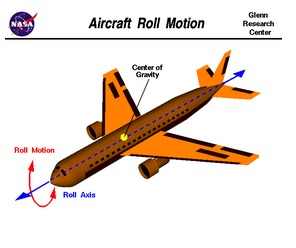
\includegraphics[height=6cm, width=80mm]{pics/roll1.jpg} 
			\caption{Example of Roll}
		\end{figure}
		\item Flight dynamics: angles of rotation in three dimensions around a vehicle's center of mass. These include yaw, pitch, and roll. Note: all references to "clockwise" and "counter-clockwise" are described from the user's perspective of his hand.
\end{itemize}


\section*{Introduction}

A Parrot AR Drone (Figure 4) is a radio-controlled flying quadcopter helicopter, which receives flight instructions via a Wi-Fi connection. The user interacts with the drone by sending it instructions from an Android or iOS device. All a user has to do is connect to the Wi-fi hotspot generated by the AR Drone and issue commands via the interface on the mobile device. The AR Drone is capable of executing instructions such as an autonomous take-off and landing, movement along the coordinate plane, rotation to its left and right, and hovering in place. With all of this functionality, these drones may be used for many different purposes, such as delivering packages or using its built-in camera to record videos and take pictures. The default interface which the developers of the Parrot AR Drone designed for controlling the quadcopter is an application that can be run on mobile devices that support either iOS or Android. Using this interface, however, proved to be very difficult to control the quadcopter properly when tested.
        
\begin{figure}[H]
	\centering
	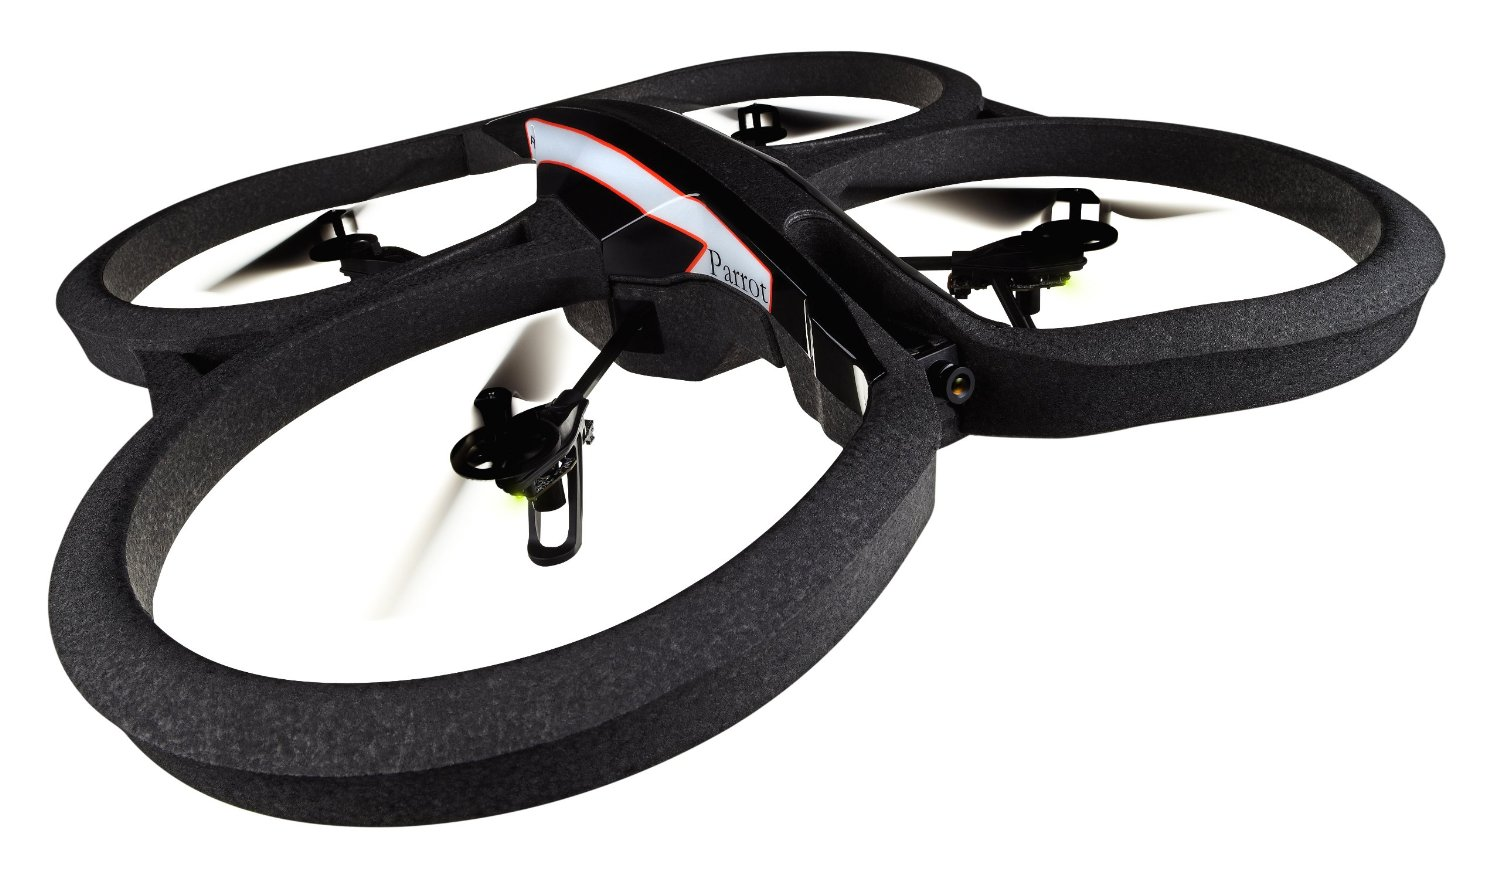
\includegraphics[height=6cm,width=90mm]{pics/drone.jpg} \\
	\caption{The Parrot AR Drone 2.0}
\end{figure}
	
The Leap Motion Controller (Figure 5) is a small, USB-sized device that is capable of tracking both hands of a user as well as all 10 fingers with great precision and speed. The controller contains LED lights and camera sensors which are constantly scanning a hemi-spherical volume with a diameter of 1 meter  and centered on the device, recording information, and sending data to the computer. The controller's software contains listeners which are able to recognize different hand gestures, such as circling, swiping, key tapping, screen tapping, and other movement of the user's hand. Most importantly for this study, the controller outputs data indicating the position of the hand, including the hand's roll, pitch, and yaw with respect to the device's sensors. With an easy-to-use application programming interface (API), this controller allows developers to receive information about a user's hands and fingers and analyze/manipulate this information as they wish.

\begin{figure}[H]
	\centering
	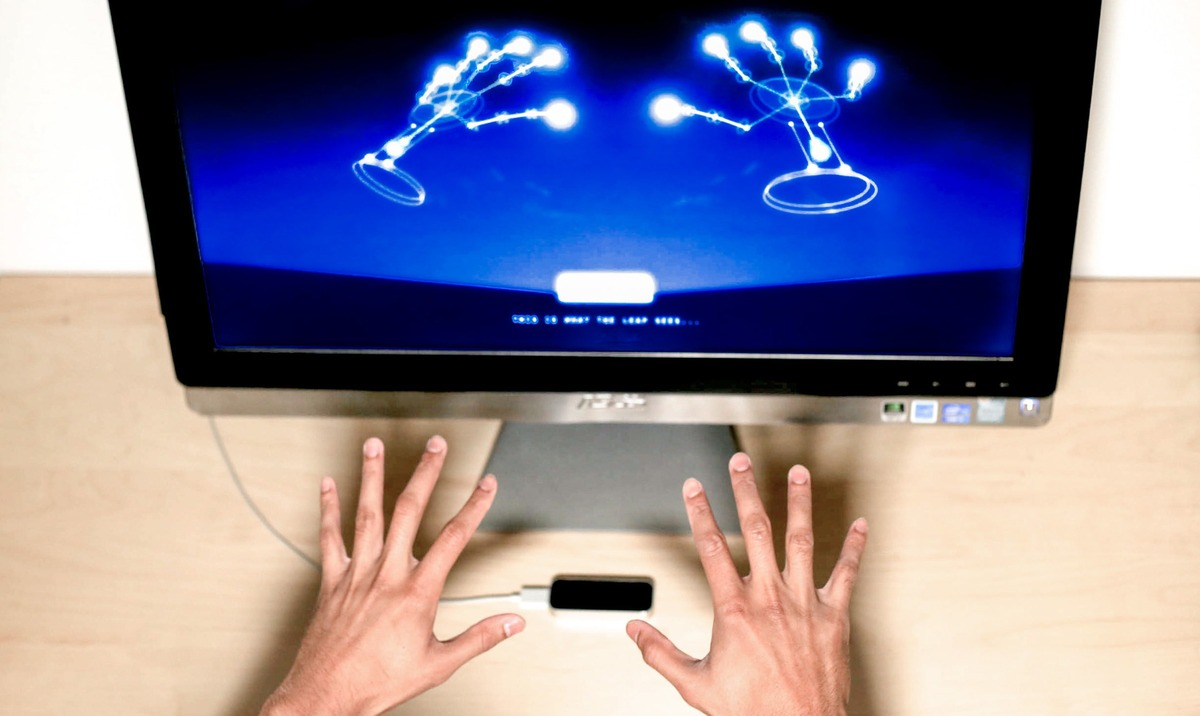
\includegraphics[height=6cm,width=90mm]{pics/leap.jpg}
	\caption{The Leap Motion}
\end{figure}

 
In this study, the Leap Motion Controller is integrated with the Parrot AR Drone, creating a new interface for users to control the drone's flight with. This newly developed interface strives to provide users with a simpler, more stable, and more natural flight control experience. Our interface allows users to control the AR Drone using basic hand gestures that are interpreted as flight instructions. Stabilization algorithms are also implemented to clearly define the user's hand gestures, allowing the interface to easily interpret the gestures as commands. After receiving input from the user, our interface analyzes and manipulates this information before sending instructions to the AR Drone. Our System Block Diagram outlines this in Figure 6. In Figure 7, our System Flow Chart is shown. This flow chart displays the decisions that the system makes based on the inputs it gets from the Leap Motion. Initially, the system checks to see if a hand is present. If it is, then the moving average algorithm will execute. Once that algorithm completes, the Drift Test algorithm executes. These two algorithms are part of the "Stability Algorithm" section of the Block Diagram in Figure 6. Once those two algorithms are completed, then the decision tree is entered so the system can figure out what command to send to the AR Drone.  The remaining decision structures in the Flow Chart belong to the "Translate data into instructions" section of the Block Diagram. Once all the decisions have been considered, then the Leap Motion delivers a new set of frames and the Flow Chart goes back to the "Start" step.

\vspace{3cm}

\begin{figure}[H]
	\centering
	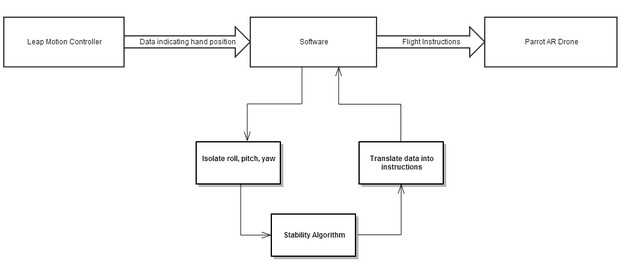
\includegraphics[height=6cm,width=140mm]{pics/blockDiagram1.jpg}
	\caption{System Block Diagram}
\end{figure}


\begin{figure}[H]
	\centering
	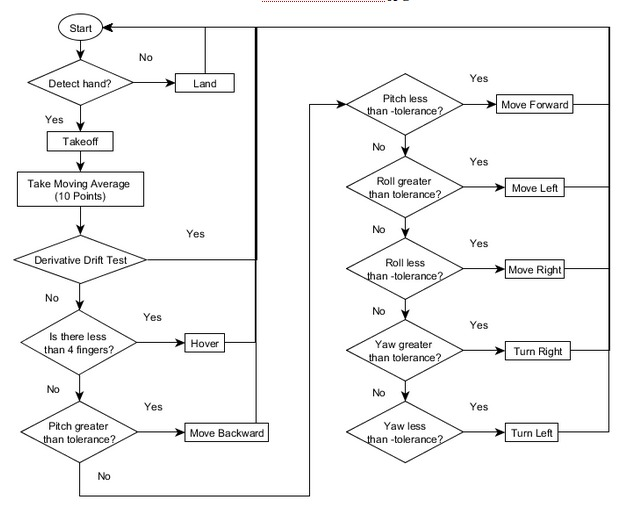
\includegraphics[height=10cm,width=130mm]{pics/controlFlowChart.jpg}
	\caption{System Flow Chart}
\end{figure}


\section*{Language Selection}

The selection of software environment was based on the performance requirements of the study, ease of implementation, and development speed. Python was chosen as the best language to use because of the availabilities of toolsets as well as open source libraries concerning leap motion data and sending instructions to the drone. The leap motion library packages raw Leap Motion data into a python object called a "frame"\cite{cit9}. The library that helped send instruction to the drone wrapped the raw hex instructions used to control the drone into Python objects. We found that Python's execution speed is within an acceptable range of responsiveness, allowing the pilot to maneuver the AR Drone without any observable delays. After investigating a few options such as Java and C++, we decided to implement the Drone interface in Python.

\section*{Gesture Selection}

Six basic gestures were used to create the interface for the Drone. These are the left and right positions, the forward and backwards positions, and the rotate left and rotate right positions. These positions were selected since the user can move his hand in the same manner as the drone can fly. In other words, there is a one-to-one correspondence between our six defined gestures and the flight patterns of the Drone. In addition, the gestures are not difficult to form and are intuitive for the user.  Each of the positions consists of holding the hand flat with the fingers held close together, and then rotating or tilting in the six directions to generate our defined states. The gestures for the study are shown and defined below.

\begin{itemize}

		\item Gesture: a placement of the hand in the space around the Leap Motion. Defined by degrees of rotation of the hand from a standard placement. All gestures recognized by the system should imitate a position similar to that of the hand when placed flat on a table. 
		\item Drone interface: set of mappings of hand gestures to the AR Drone's flight dynamics which is presented to the user. 
		\item Mean (Hover,neutral) position: State defined with the plane of the palm parallel to the ground.The normal vector from the plane of the palm should be pointing towards the and should be perpendicular to the ground. The hand should be held approximately 10 centimeters above the Leap Motion. \\
		\begin{figure}[H]
			\centering
			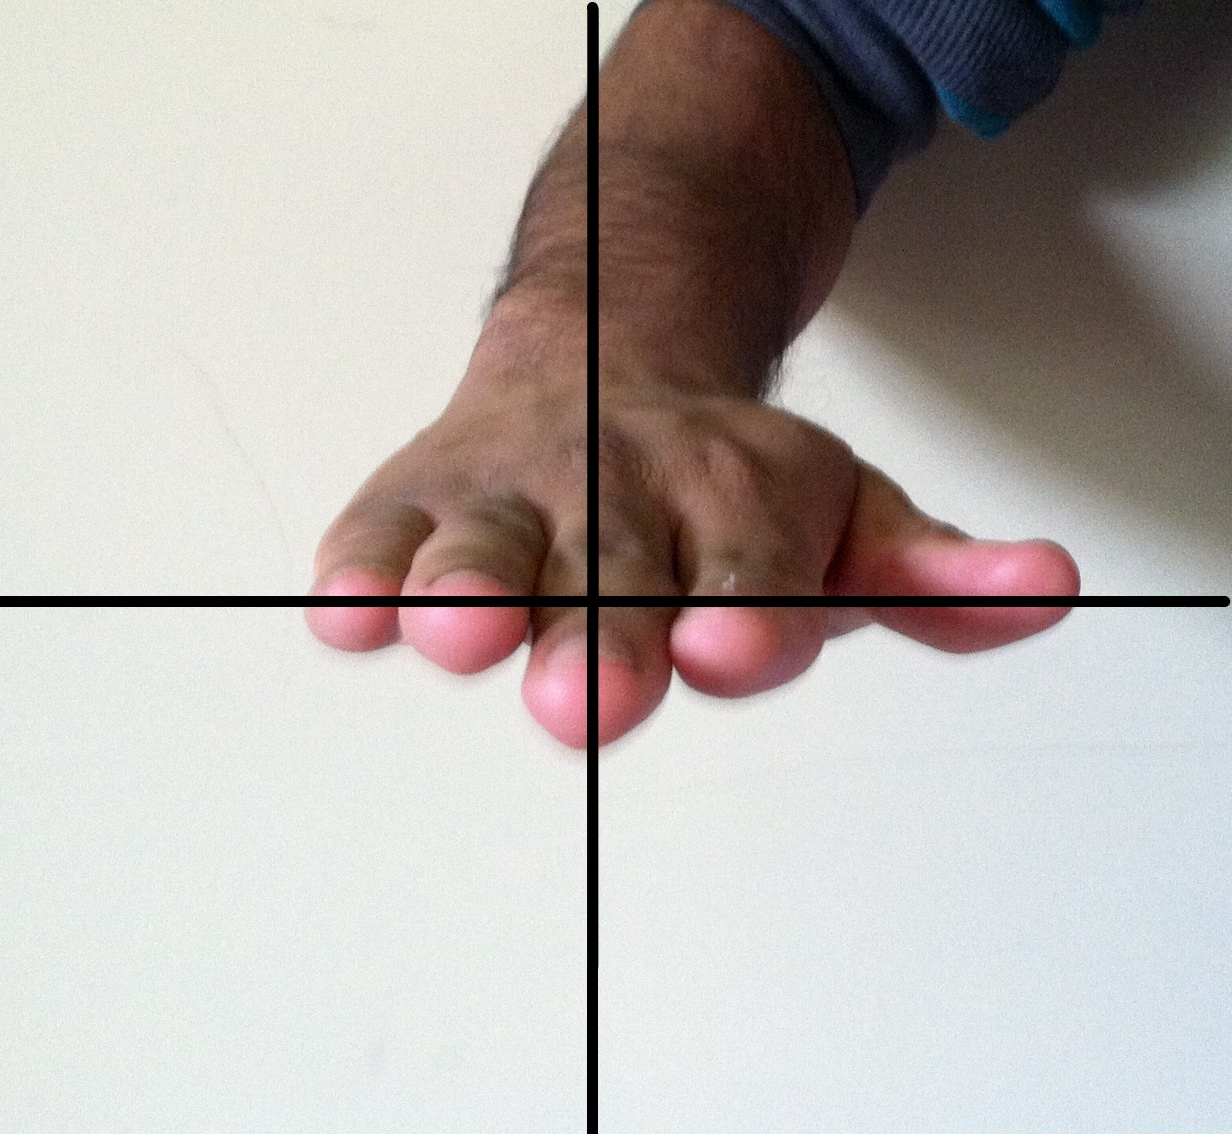
\includegraphics[height=6cm, width=80mm]{pics/mean.jpg} 
			\caption{The Mean Position}
		\end{figure}
		\item Left position: State defined with the normal vector of the palm rotated counter-clockwise along the longitudinal axis by greater than 4 degrees measured from the mean position. \\
		\begin{figure}[H]
			\centering
			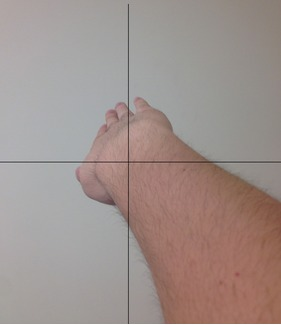
\includegraphics[height=6cm, width=80mm]{pics/left.jpg} 
			\caption{The Left Position}
		\end{figure}
		\item Right position: State defined with the normal vector of the palm rotated clockwise along the longitudinal axis by less than -4 degrees measured from the mean position. \\
		\begin{figure}[H]
			\centering
			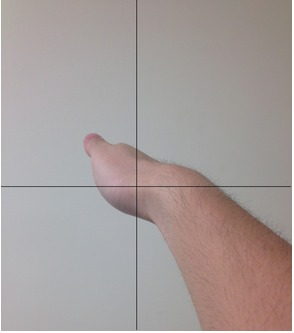
\includegraphics[height=6cm, width=80mm]{pics/right.jpg} 
			\caption{The Right Position}
		\end{figure}
		\item Forward position: State defined with the normal vector of the palm rotated clockwise along the lateral axis by greater than 6 degrees from the mean position. \\
		\begin{figure}[H]
	 		\centering
			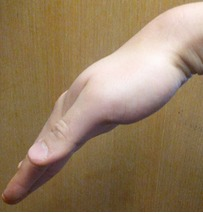
\includegraphics[height=6cm, width=80mm]{pics/forward.jpg} 
			\caption{The Forward Position}
		\end{figure}
		\item Backward position: State defined with the normal vector of the palm rotated counter-clockwise along the lateral axis by less than -6 degrees from the mean position.  \\
		\begin{figure}[H]
	 		\centering
			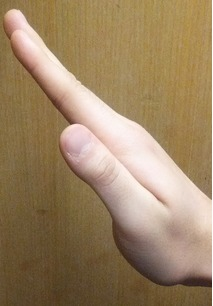
\includegraphics[height=6cm, width=80mm]{pics/backward.jpg} 
			\caption{The Backward Position}
		\end{figure}
		\item Rotate left position: State defined with the normal vector of the palm rotated counter-clockwise along the normal axis by greater than 12 degrees from the mean position. \\
		\begin{figure}[H]
			\centering
			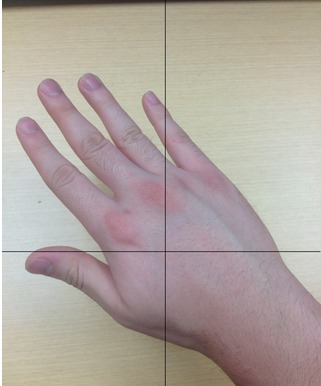
\includegraphics[height=6cm, width=80mm]{pics/rotateLeft.jpg} 
			\caption{The Rotate Left Position}
		\end{figure}
		\item Rotate right position: State defined with the normal vector of the palm rotated counter-clockwise along the normal axis by less than 12 degrees from the mean position. \\
		\begin{figure}[H]
			\centering
			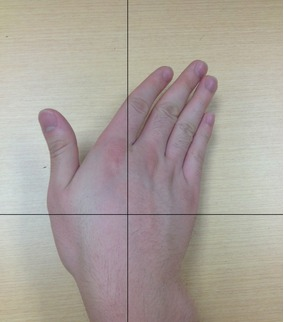
\includegraphics[height=6cm, width=80mm]{pics/rotateRight.jpg} 
			\caption{The Rotate Right Position}
		\end{figure}
	
\end{itemize}

\section*{Overview of Approach}

The system in this study consisted of three distinct portions; the Leap Motion device, our own processing software, and the interpretation by the AR Drone. As the block diagram in Figure 6 shows, the software that we wrote acts as an controller between the Leap Motion and AR Drone devices and uses a series of steps to transform the data generated by the Leap Motion into commands that the AR Drone can execute.

Our software consists of three subsections; isolation of the data about the three flight dynamics of the hand, stabilization the three sets of data and recognition of different hand states, and a decision structure about the command to be sent to the Drone. The process is started by turning on the Leap Motion and running our software. The Leap Motion begins collecting data about hands in its area of detection and begins creating frames of data. Next, the Leap forwards the frames to the controller software, which unpacks the roll, pitch, and yaw data. The stabilization and recognition algorithms are run on the received data, and then the decision tree in Figure 7 is traversed to decide what control message to send. Finally, the controller software forwards the control message to the AR Drone, which understands what flight pattern is desired, and the drone flies in the appropriate direction. Once the command is interpreted, then the Leap Motion collects a new frame of data. This process continues until the user terminates the process.

\section*{Data Collection}
\subsection*{Categorization}

Data is collected from the Leap Motion Controller using Leap Motion's Software Development Kit (SDK). This SDK contains many listeners which receive information from the sensors in frames, which are snapshots of the hand taken at specific intervals. Listeners are software objects that execute certain instructions once an event occurs. For example, a motion-sensor can be thought of as a physical version ofa listener. The sensor will continually wait until movement occurs; once the movement does occur, the sensor will light up. Thus, the motion-sensor "listens" for movement. For our study, the Leap Motion was set to generate 300 frames of hand data per second. The SDK provided us with several listeners that collected different types of data, and we modified those listeners to collect the attributes we were looking for. The listeners most relevant to the system were  \textbf{on\_connect()}, \textbf{on\_frame()}, and \textbf{on\_focus\_gained()}. \textbf{On\_connect()} could be used to send commands to the drone as soon as the script connected to the Leap Motion. However, this listener was discarded because it would continuously send messages to our script even when frame data is not present. The \textbf{on\_focus\_gained()} listener allows the caller to send commands every time the window where the script is running gains the focus. This listener was also discarded because the stream of commands to the script could be interrupted if the focus on the window is lost. The remaining listener, \textbf{on\_frame()}, allows the caller to execute commands every time that the Leap Motion receives a frame of data. This listener was chosen because it enables the system to respond only when relevant data has been gathered. In the other two listeners,  the execution of commands is dependent on either another factor such as focus, or the maintenance of a connection. The use of these two listeners would slow down the system in two different ways. In the case of \textbf{on\_connect()}, the system would get bombarded with control messages which may or may not contain frame data. Having the system unpack messages which do not contain any relevant information is a waste of resources, and results in less efficiency. The \textbf{on\_frame()} listener is inefficient because data is only transmitted as long as the focus on the window is maintained. The user can make any gesture he wants, but those commands will never get sent or processed if the computer's focus on the window is lost. Thus, having the system depend on the focus is unpredictable and inefficient, so we discarded it. Due to the drawbacks of the \textbf{on\_connect()} and \textbf{on\_frame()} listeners, the \textbf{on\_frame()} listener was chosen to receive data from the Leap Motion.

Once the script connected to the Leap Motion, it was able to receive and parse the frame data that was being sent from the device. Each frame is designed to contain information about the roll, pitch, and yaw of the hand in degrees. The degree measurements in each case are taken as the angle measured between the normal vectors of an arbitrary position and the mean position. A sample frame is shown in Figure 15.

\begin{figure}[H]
	\centering
	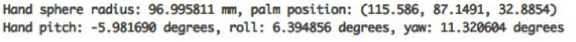
\includegraphics[height=1cm,width=130mm]{pics/frameData.jpg}
	\caption{Sample frame for the Move Right gesture}
\end{figure}

\begin{figure}[H]
	\centering
	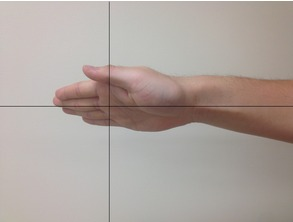
\includegraphics[height=6cm,width=90mm]{pics/correspondingHand1.jpg}
	\caption{Side view of the Move Right gesture}
\end{figure}

\begin{figure}[H]
	\centering
	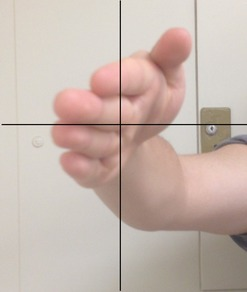
\includegraphics[height=6cm,width=90mm]{pics/correspondingHand2.jpg}
	\caption{Front view of the Move Right gesture}
\end{figure}

Once the frame data is retrieved, we parse each frame for the degree measurements in each of the six positions shown in Figures 8 through 14.

The frame structure shown in Figure 15 was used to collect data about the six positions defined for our system. Each position was held for a period of 10 seconds, and the degree measurements for each flight dynamic were recorded from the frame data. The theoretical angle of 45 degrees from the neutral position was used as a reference point, and variations from that position were measured. We know that the human hand does not stay absolutely still when held in a position, so degree measurements were taken over a period of time to observe how much variation the hand produced. A set of frames were generated during the 10 second period of holding a particular position, and this set contained all the degree measurements taken by the Leap Motion over the 10-second time period. Each frame from every set was parsed and the measurements for the intended flight dynamic were placed in an array that will be passed to to the Moving Average algorithm. For example,  all the roll measurements from the Right position were parsed from the frames because the intended flight dynamic for that position is the roll. Similarly, we parsed the frames for all the pitch measurements from the Forward and Backward positions because the pitch is the intended flight dynamic. We continued this process for the remaining gestures to collect degree measurements for the rest of the states. Once all the degree measurements were correctly parsed from the frames, the data set was passed to the stabilization and recognition algorithms for processing.


\subsection*{Stabilizing Flight}

Each state is defined by an offset of specific degrees from the mean position of the hand, depending on the desired state. The mean position is defined with the hand hovering directly over the Leap Motion with the palm facing towards the floor, as shown in Figure 8. Move left and move right, which are shown in Figures 9 and 10, are determined by the offset of roll from the mean position. Move forward and move back, shown in Figures 11 and 12,  are determined by the offset of pitch from the mean position. Finally, turn left and turn right are determined by the offset of yaw from the mean position and are demonstrated in Figures 13 and 14. For roll, the degree measurements are made relative to the rightmost part of the hand. Positive degree measurements are measured with the unit circle as a reference. The measurement for pitch is analogous, but the fingertips are used as the reference. Finally, yaw is also measured using the fingertips, with zero degrees being the direction directly in front of the user.

After collecting some degree measurements for each state, we conjectured that the variations in position could be caused by two types of involuntary hand movements: Hand Shaking and Hand Drifting.  Hand Shaking occurs because it is impossible for the pilot to keep his hand completely still, so there will always be some degree of "shaking" over the Leap motion. Shaking is characterized by slight rotations of the hand around a particular gesture in all three flight dynamics. The rotations are very swift and tend to reverse direction quickly. During these rotations, the hand is moving fast but does not move very far from our desired hand gesture.  Hand Drifting occurs when the pilot is focusing so much on the AR Drone that he does not notice that his hand seems to be rotating slightly, resulting in unintentional movements in the drone's flight. A characteristic of drifting is slow rotational movement of the hand that deviates away from the mean position; in other words, the pilot's hand will deviate to an unintentional flight instruction - for example, a pilot's hand might initially be in the "move left" state but gradually move toward the "move right" state without the pilot being aware of this shift. The system must account for this unintentional movement caused by human error and understand that it should not recognize a different state because of it. 

To further understand Hand Shaking, we collected sample sets of degree measurements from the Leap Motion for each defined state. 3000 samples were collected from each gesture over a period of 10 seconds for each of the desired positions, and the results were stored in a text file using the comma-separated-value (CSV) format.

\begin{figure}[H]
	\centering
	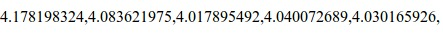
\includegraphics[height=1.5cm,width=130mm]{pics/CSV.jpg}
	\caption{An example of comma separated values}
\end{figure}


We picked the CSV format for our data, because of its ease of import into MATLAB, a high-level language for mathematical analysis, numerical computation, and data visualization.  We can use the different tools and functions of MATLAB to understand our data.
 
The goal in eliminating the "shaking hand" problem was to match the Leap Motion data to a particular probability distribution, and then utilize that distribution to remove any outliers from our data set. Once the outliers were eliminated, we marked certain points in the distribution within which a state could be recognized. Our initial hypothesis was that the data collected will be normally distributed, such as in Figure 19. The normal distribution plots the frequency with which a specific data point is measured, and it describes a set of data that tends to a central value, and no bias to left or right \cite{cit3}.

\begin{figure}[H]
	\centering
	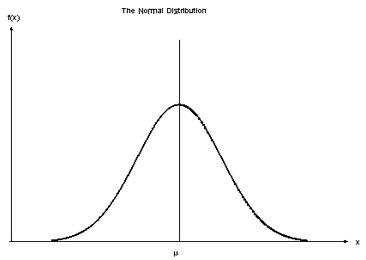
\includegraphics[height=6cm,width=90mm]{pics/genNormalDist1.jpg}
	\caption{The Normal Distribution}
\end{figure}

Using a normal distribution to analyze our data presents several advantages. First, the distribution is characterized by a mean value and a standard deviation from that mean value. The mean value signifies the intended degree of the pilot's hand, and the standard deviation is the offset caused by the shaking of the pilots hand. For example, if the pilot intends to move right, the pilot will move his hand past the tolerance of the hover state towards the roll state. Using the data measured from this new position of the pilot's hand, the drone will move to the right with a velocity which is calculated using the roll degree of the hand. However, due to the shaking of our hand and the noise of the Leap Motion, measurements that deviate slightly from the mean will also be recorded. These variations are frequent and are localized around the mean position, because it is very unlikely that large degrees of variations will be recorded. However, as one moves further from the mean position, the frequency of the variations decrease. This occurs because the probability of a great variation being recorded diminishes as the degree value is increased or decreased. If the hand is supposed to be held at 10 degrees, then the majority of the measurements will fall within a range of 5 to 15 degrees. In this case, a variation of 100 degrees from the mean position is very unlikely, and the normal distribution can predict this by showing a small number of measurements taken at 100 degree variation from the mean. Thus, the degree of variation from the mean continually decreases as one moves further and further away from the mean value, which is an expected behavior of this distribution. 

Second, we can use the standard deviation of the distribution to determine how widely distributed the data set is. The standard deviation quantifies the notion of "hand shaking" because it shows the frequency of variations from the mean position. With this characteristic, we can decide how much of the data we would like to include in our analysis. We can use a specific multiple of the standard deviation to create threshold values between which data can be recognized as significant. For example, we can decide to set the thresholds at half a standard deviation on either side of the mean. This means that any data point that is recorded between those two threshold values, say 40 degrees and 50 degrees, will be recognized as significant. Using the standard deviation, we set certain threshold values for each gesture such that any values that fall within that range will correspond to the correct gesture.

 The thresholds are used to mark the maximum variation that a particular state accepts. If the hand is positioned outside of the threshold value for enough time, then the system will not recognize the gesture. Since the gestures are uniquely defined by the threshold values, the hand gesture can be uniquely mapped to a flight pattern. Once the gestures get mapped, a simple decision structure can decide what command gets sent to the AR Drone.

As an initial test, we graphed our data using histograms to see if the shape of the data seemed to close enough to the normal distribution. A histogram is a graphical representation of data which tabulates the frequency of data points over intervals of adjacent rectangles, otherwise known as bins \cite{cit5}. We created histograms for every position, and found mixed results. 

Figures 20-26 show the histograms for the different positions. The basic criteria that we used to find gaussian shaped distributions were the presence of a single, distinct mean value and a bell-shaped curve that eventually diminished to zero. Using this criteria, we found that some of the histograms closely resembled the normal distribution, while others were only somewhat related. For example, the histogram for the left position appeared to be centered at 31 degrees, but had data points skewed to the left. It did have two tails that diminished to zero at around 28 and 32 degrees, but the sizes of these tails were also affected by the negative skewness.  However, the distribution of the data was similar to the bell-shape of the Gaussian distribution and had a prominent mean, so this set strengthened our hypothesis. On the other hand, the Forward data set showed a distribution very different to the normal distribution. There appeared to be four different peaks in the frequencies, with three of the peaks clustered within a range of four degrees and centered at approximately -108 degrees. These four peaks were unexpected, and their placement in relation to the degree measurements was too erratic. We could not confidently say that the data for this set could be described by a Gaussian distribution. The trend in the histograms showed that each sample set would show either one prominent mean or three to four less prominent means. Due to this trend, we could not confidently conclude that each of the samples could be approximated as a normal distribution. We also concluded that histograms are not an entirely reliable test of normality. An appearance similar to a particular distribution is not enough, since it could be modeled by a function similar to but not exactly the same as that for a bell curve. Unless we are absolutely sure that the data set could be matched to a distribution, we cannot make any conclusions based solely off of a histogram for the data set. Thus, we turned to more rigorous, mathematical tests to confirm the normality of our data.

\begin{figure}[H]
	\centering
	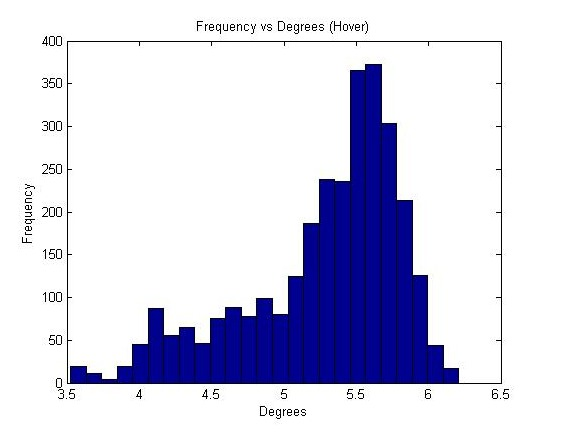
\includegraphics[height=6cm,width=90mm]{pics/hoverHistogram1.jpg}
	\caption{This is the histogram of our hand in hover position. Due to the nature of this state being the easiest to maintain, we feel that this is the most accurate sample for "drifting". It looks to be a Gaussian distribution with a pronounced mean at 5.5 and the tails diminishing the further it is away from it.}
	\centering
\end{figure}

\begin{figure}[H]
	\centering
	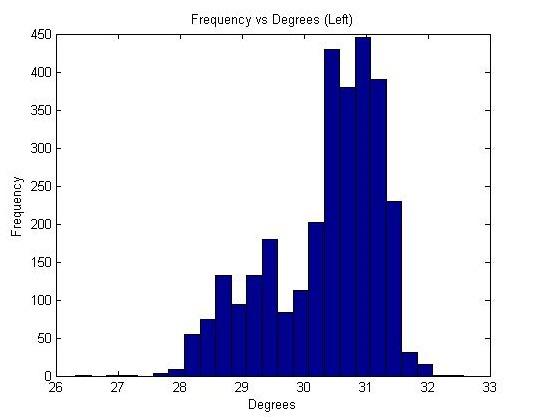
\includegraphics[height=6cm,width=90mm]{pics/leftHistogram1.jpg}
	\caption{This is the histogram for our hand in the move left state. It is only supposed to take into account the degrees for roll, therefore the data in this histogram is a graphical interpretation of roll in degrees.  As can be seen, the data's mean is around 31 degrees, and diminishes on the tails.}
\end{figure}

\begin{figure}[H]
	\centering
	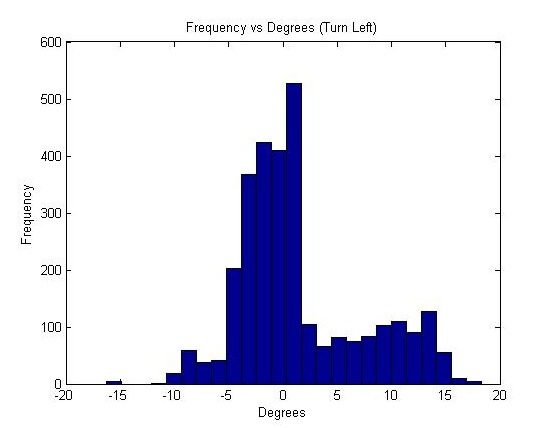
\includegraphics[height=6cm,width=90mm]{pics/turnLeftHistogram1.jpg}
	\caption{This is the histogram for our hand in the turn left state. It is only supposed to take into account the degrees for yaw, therefore the data in this histogram is a graphical interpretation of yaw in degrees.  As you can see, the data's mean is around 0 degrees, and diminishes on the tails. Movement-wise, yaw is the most difficult for the pilot and is likely to give us shaking noise.  From our data it can be seen that the range of error is bigger than the other frames of different positions.}
\end{figure}

\begin{figure}[H]
	\centering
	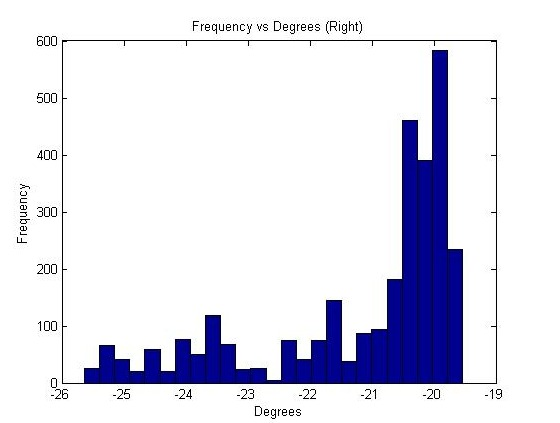
\includegraphics[height=6cm,width=90mm]{pics/rightHistogram1.jpg}
	\caption{This is the histogram for our hand in the move right state. It is designed to account for the degrees for roll, therefore the data in this histogram is a graphical interpretation of roll in degrees.  As can be seen, the data's mean is around -20 degrees, and diminishes on the tails. 
Our data is skewed towards the right of the sample set.

s skewed on one side, there is more deviation towards the more negative degrees, and move right is represented by negative degrees.  Thus it means the the pilot's hand is shaking towards the right.}
\end{figure}

\begin{figure}[H]
	\centering
	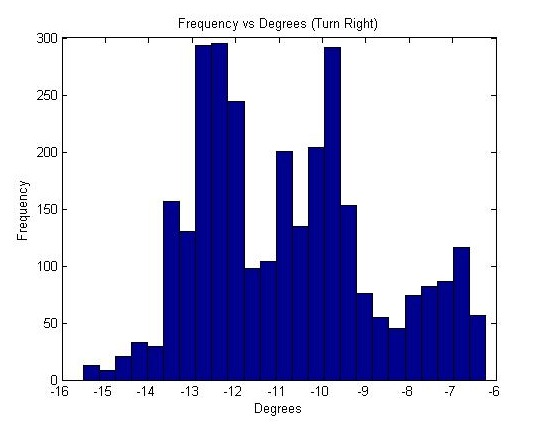
\includegraphics[height=6cm,width=90mm]{pics/turnRightHistogram1.jpg}
	\caption{This is the histogram for our hand in the turn right state. It is only supposed to take into account the degrees for roll, therefore the data in this histogram is a graphical interpretation of roll in degrees.  As can be seen, the data's mean is around -13 degrees, and diminishes on the tails. Movement wise, yaw is the most difficult for the pilot and is likely to give us shaking noise.  From our data it can be seen that the range of error is bigger than the other frames of different position.}
\end{figure}

\begin{figure}[H]
	\centering
	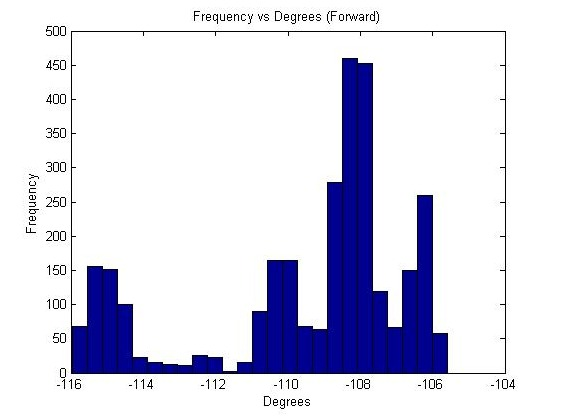
\includegraphics[height=6cm,width=90mm]{pics/forwardHistogram1.jpg}
	\caption{This is the histogram for our hand in the turn right state. It is only supposed to take into account the degrees for roll, therefore the data in this histogram is a graphical interpretation of roll in degrees.  As can be seen, the data's mean is around -13 degrees, and diminishes on the tails. Movement wise, yaw is the most difficult for the pilot and is likely to give us shaking noise.  From our data it can be seen that the range of error is bigger than the other frames of different position.}
\end{figure}

\begin{figure}[H]
	\centering
	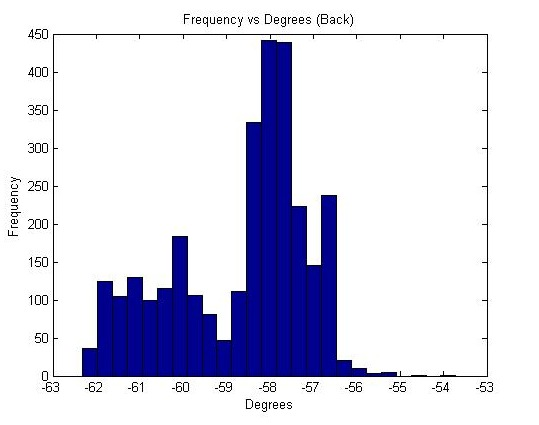
\includegraphics[height=6cm,width=90mm]{pics/backwardHistogram1.jpg}
	\caption{This is the histogram for our hand in the move back state.It is only suppose to take into account the degrees for pitch, therefore the data in this histogram is a graphical interpretation of pitch in degrees.  As can be seen, the data's mean is around -58 degrees, and diminishes on the tails. Notice that the data is skewed more towards the more negative degrees, meaning that the hand is shaking towards the move back state more.} 

\end{figure}


The data generated by the Leap Motion is unfiltered; this means that no smoothing algorithms are applied internally by the device before getting packaged into frames \cite{cit11}. So, the data that the script manipulates is unadulterated, raw data. Because of this, it is up to the developer to search for and remove extreme values in the distribution. In addition, histograms like the ones shown in the figures above accurately depict the measurements of the hand since no filtering is done. Thus, we can confidently use a histogram to determine what kind of gesture is being performed. For example, the gesture in Figure 13 is indicating the Right gesture since a majority of the points are concentrated around the -20 degree point. The feed of raw data from the Leap Motion gives the developer an advantage because he is allowed to implement whatever filters he likes. The developer can then emphasize whatever data points he wants, be they the central values or the extreme values.

After reading some publications regarding normality testing, we came across four tests that were reputed to be the best. These were the Kolmogorov-Smirnov test, the Lilliefors test, the Anderson-Darling test, and the Shapiro-Wilks test, Although all of these test for normality, each processes the data in a different way.

The Kolmogorov-Smirnov test is a type of empirical distribution test (EDF), and it calculates the largest vertical difference between empirical data and hypothesis data \cite{cit8}. That means we need a set of data which we know is comparable to our empirical data, but in our case we cannot do that because we don't know the hypothetical data for our hand positions. 

The Lilliefors test is similar to the Kolmogorov Smirnov test because it is also a type of EDF. However instead of knowing the hypothetical data, the hypothetical data is calculated from the empirical data. Making this test desirable for us because we do not know the hypothetical data for our hand positions \cite{cit7}

The Anderson-Darling test is also a variation on the Cramer Von Mises (CVM) test, and it gives more weight to the tails of the distribution than does the CVM test. The advantage of this test is that it is supposed to be the most powerful of EDF test \cite{cit10}.


The Shapiro-Wilks test is based on a null hypothesis which assumes that the data being tested is no different than data drawn from a normal distribution. An alpha level, which is a measure of statistical significance, is then set to a value of .05. Once this value is chosen, the test is run and consequently returns a p-value. This p-value is compared to the chosen alpha level to determine whether the null hypothesis should be rejected; if the p-value is greater than the alpha level, then the null hypothesis cannot be rejected. If the p-value is less than the alpha value, then the null hypothesis is rejected \cite{cit2}.


After researching these tests, we decided to use the Shapiro-Wilks test because we found it to be the most powerful. We based this decision on a paper written by Razali \& Wah \cite{cit1} which compares the power of the four formal tests. The power of a formal normal distribution is defined as the probability that the test correctly rejects the null hypothesis when the null hypothesis is false. 

Razali and Wah used power comparisons which were obtained through Monte Carlo simulation, the data for which was generated by various sample sizes and alternative normal distributions with varying levels of kurtosis and skewness.  Skewness quantifies the symmetric qualities of the distribution, and kurtosis quantifies how closely the shape of the distribution matches the Gaussian.  

In our case, the null hypothesis is that the data follows a normal distribution, and the power is the probability that this hypothesis is rejected when our data is not normally distributed.  

We show the power comparisons of 2 plots of power for symmetric distribution and 2 plots of power for asymmetric distribution from Razali and Wah's paper. The Beta, Laplace, and Gamma distributions were chosen arbitrarily as examples to illustrate the tests.

The following are plots of power for the Symmetric Distributions Beta(2,2) and Laplace(0,1):

\begin{figure}[H]
	\centering
	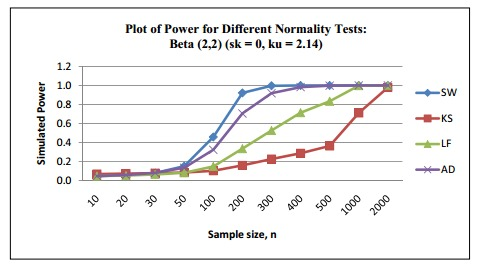
\includegraphics[height=6cm,width=90mm]{pics/razali1.jpg}
	\caption{Razali and Wah's power comparison using the Beta(2,2) distribution. "SW" represents the Shapiro-Wilk test, "KS" represents the Kolmogorov-Smirnov test, "LF" represents the Lilliefors test, and "AD" represents the Anderson-Darling test}
\end{figure}

\begin{figure}[H]
	\centering
	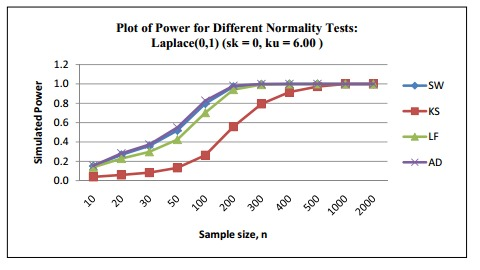
\includegraphics[height=6cm,width=90mm]{pics/razali2.jpg}
	\caption{Razali and Wah's power comparison using the Laplace(0,1) distribution. "SW" represents the Shapiro-Wilk test, "KS" represents the Kolmogorov-Smirnov test, "LF" represents the Lilliefors test, and "AD" represents the Anderson-Darling test}
\end{figure}

The following are plots of power for the Asymmetric Distributions Gamma(4,5) and Gamma(1,5) distributions:

\begin{figure}[H]
	\centering
	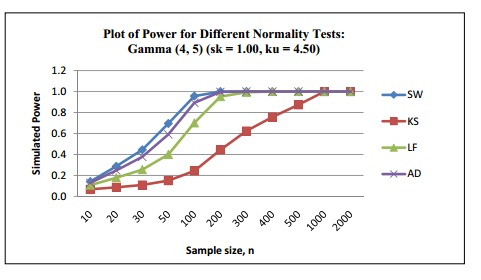
\includegraphics[height=6cm,width=90mm]{pics/razali3.jpg}
	\caption{Razali and Wah's power comparison using the Gamma(4,5) distribution. "SW" represents the Shapiro-Wilk test, "KS" represents the Kolmogorov-Smirnov test, "LF" represents the Lilliefors test, and "AD" represents the Anderson-Darling test}
\end{figure}

\begin{figure}[H]
	\centering
	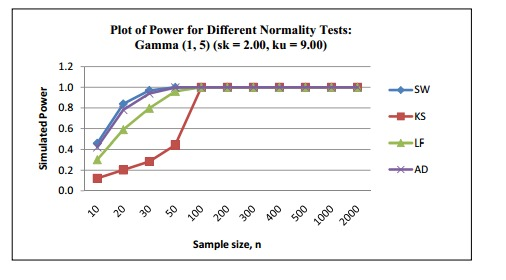
\includegraphics[height=6cm,width=90mm]{pics/razali4.jpg}
	\caption{Razali and Wah's power comparison using the Gamma(1,5) distribution. "SW" represents the Shapiro-Wilk test, "KS" represents the Kolmogorov-Smirnov test, "LF" represents the Lilliefors test, and "AD" represents the Anderson-Darling test}
\end{figure}

As is shown by the results of the comparison tests, the Shapiro-Wilks test is the most powerful out of the four tests with the various sample sizes and distributions (Razali \& Wah 2011). For every distribution tested, the Shapiro-Wilks test rose to the maximum power level faster than any of the other tests. Another observation is that the Shapiro-Wilks test was at the maximum power level for several sample sizes smaller than the one being considered. For example, by a sample size of 500, the Shapiro-Wilks test had executed with maximum power for the 300- and 400- sized sets before it for every distribution tested. Other tests were still increasing in power for the 300- and 400- sized sets, and they only reached the maximum power level at a sample size of 500 or greater. From these graphs, we determined that the Shapiro-Wilks test would be the most powerful test to use because it can give us accurate normality readings for small and large sample sizes. Although the Shapiro-Wilks test is accurate for a wide range of sample sizes, we decided to use the test with a sample size of 3000. This decision was based on the rate at which the Leap Motion generates data along with the desire to ensure that the test operated at the maximum power.

Once we determined that the Shapiro-Wilks test was the ideal test of choice for our study, we used it to test our data using MATLAB. However, none of the outputs that we received returned a positive result for any of our data sets. Therefore, our hypothesis was unfortunately rejected as the P value for every sample came out to be 0.0, which is less than 0.05. (Shapiro \& Wilk 1965). 

\begin{figure}[H]
	\centering
	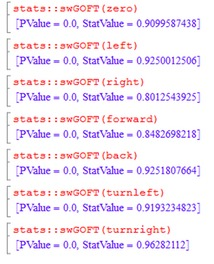
\includegraphics[height=9cm,width=70mm]{pics/swMatlab.jpg}
	\caption{Results from MATLAB's Shapiro-Wilks test}
\end{figure}

We knew that rejection of the null hypothesis was possible, but we did not expect the test to reject the null hypothesis for every data set. This seemed strange to us, so we decided to run a general distribution test in MATLAB to find out what distribution the data corresponded to.
The test matched the data sets to the General Extreme Value distribution. This distribution is characterized by a set of data which focuses on the minimum and maximum values, or the "rarities".  Since we did get a response back from this test, we decided to use one more method of confirmation: a quantile-quantile plot. Quantiles are points taken at regular intervals from the cumulative distribution function of a random variable, a function whose value is the probability that a corresponding continuous random variable has a value less than or equal to the argument of the function \cite{cit4}. Thus, the QQ (Quantile-Quantile) plot compares the quantiles of our data with the quantiles of the normal distribution The comparison tells us that the closer the data points are to the line y = x, the more likely it is that the data set came from a normal distribution.

Figure 33 shows the QQ Plot for the Left Position. As is shown by the plot, the center of the data follows the y=x line. However, the data set deviates from the line towards the tails of the plot, which indicates that there was a greater deviation from the normal distribution for those points. We saw similar behavior in the QQ plots of the other positions, but some of those plots visibly deviated more at the tail values than did the plot for the Left position. For example, the Forward position plot exhibited a great deal of variation on both the left and right tails of the distribution, much more so than the Left position plot, and a small of amount of variation around the center of the distribution. The Forward position plot contained the most deviation from the y=x line. From these plots, we confirmed that our distribution is that of the general extreme value distribution, because the tails deviated from the line thus it focuses on the minimum and maximums of our data.

Since the general extreme value distribution emphasizes the minimums and maximums of the data, we focused on including those variations. To take the tails into account, we decided to include data that fell within two standard deviations of the mean. This guaranteed that the behavior at the tail end of the distribution would be recorded and accounted for.

Using the left test, we can see that the data follows normal distribution in the middle, but does not at the minimum and maximum.  The QQ Plots for the different positions: Hover, Move Left, Move Right, Turn Left, Turn Right, Move Forward, and Move Back can be seen below.  

\begin{figure}[H]
	\centering
	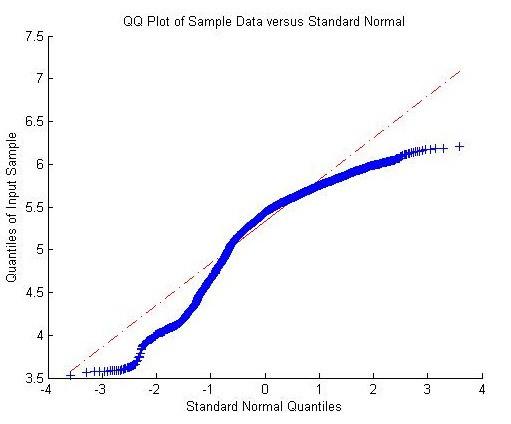
\includegraphics[height=6cm,width=90mm]{pics/qqHover.jpg}
	\caption{QQ Plot for the Hover gesture.}
\end{figure}

\begin{figure}[H]
\centering
\subfloat[extra text][QQ Plot for the Move Left gesture.] {
	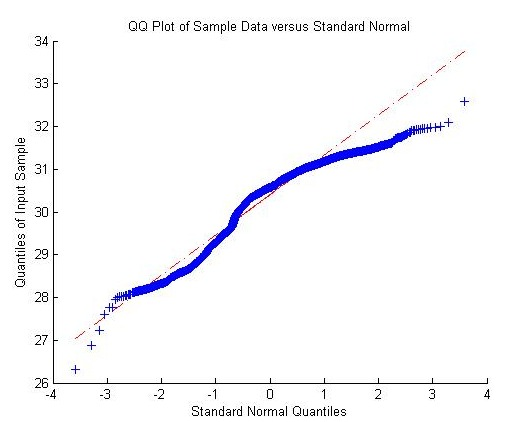
\includegraphics[width=0.4\textwidth]{pics/qqLeft.jpg}
	\label{fig:subfig1}}
	\hspace{0.5cm}
\subfloat[text][QQ Plot for the Move Right gesture.] {	
	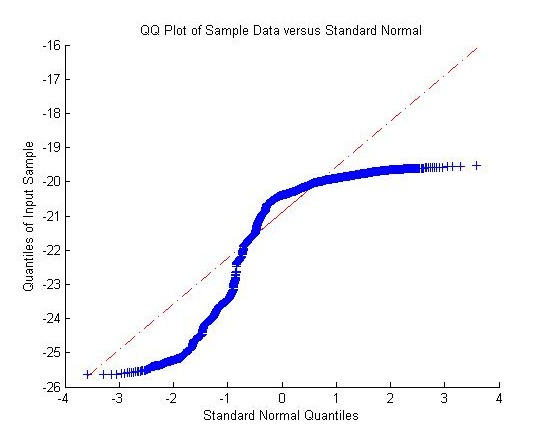
\includegraphics[width=0.4\textwidth]{pics/qqRight.jpg}
	\label{fig:subfig2}}
\end{figure}

\begin{figure}[H]
\centering
\subfloat[extra][QQ Plot for the Turn Left gesture.] {
	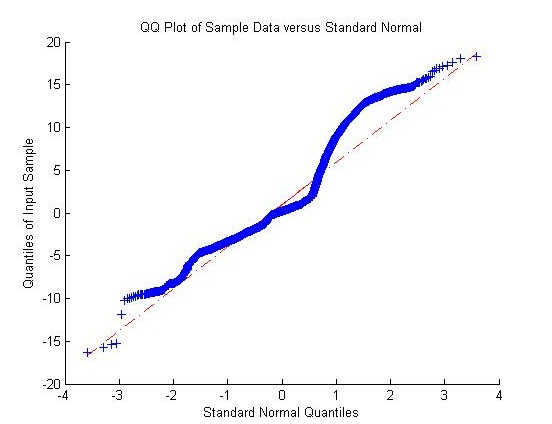
\includegraphics[width=0.4\textwidth]{pics/qqTurnLeft.jpg}
	\label{fig:subfig3}}
	\hspace{0.5cm}
\subfloat[text][QQ Plot for the Turn Right gesture.] {
	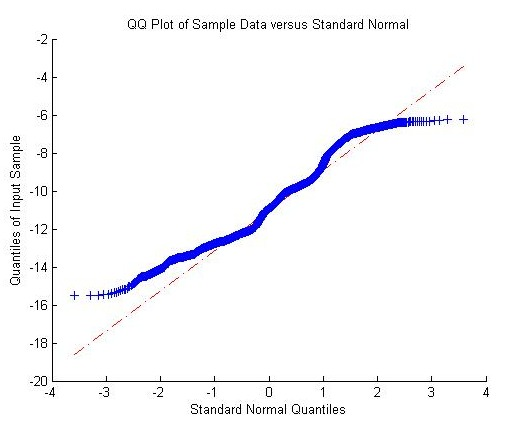
\includegraphics[width=0.4\textwidth]{pics/qqTurnRight.jpg}
	\label{fig:subfig4}}
\end{figure}

\begin{figure}[H]
\centering
\subfloat[text][QQ Plot for the Forward gesture.] {
	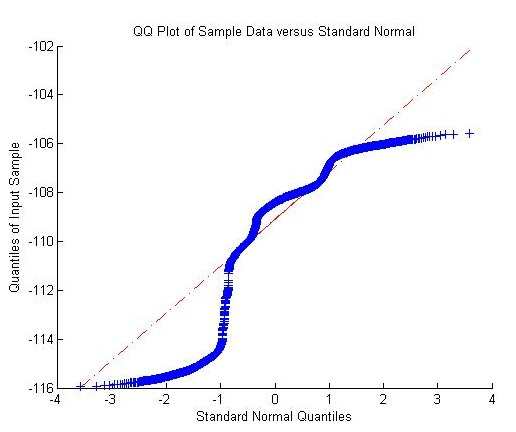
\includegraphics[width=0.4\textwidth]{pics/qqForward.jpg}
	\label{fig:subfig5}}
	\hspace{0.5cm}
\subfloat[text][QQ Plot for the Backward gesture.] {
	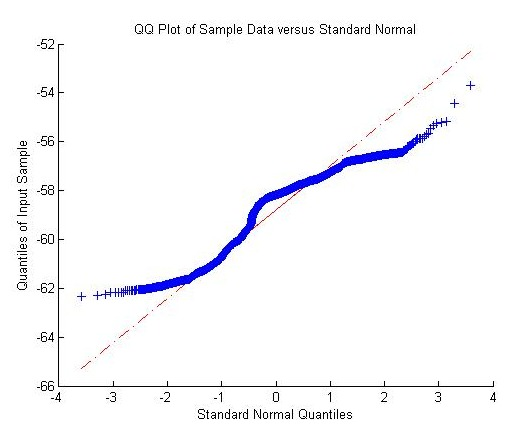
\includegraphics[width=0.4\textwidth]{pics/qqBackward.jpg}
	\label{fig:subfig6}}
\end{figure}

Armed with the knowledge that our data follows the general extreme value distribution, we determined threshold values with which the pilot's hand can shake and still be considered the correct gesture. These thresholds serve as boundary values for each state; any degree measurements recorded outside of these values will not be recognized as part of the gesture. We decided to use the value of two standard deviations on either side of the mean as our threshold values because these values would include 95\% of the data points. By doing this, we make sure that certain degrees of tilt can be tolerated, but not so much that the gesture becomes too extreme for the user. For example, the move left state could be positioned at 45 degrees from the neutral position, and angles in the range of 43 to 47 degrees will be recognized if the standard deviation is 2 degrees. The value of the deviation for each gesture is tabulated in the following table.

\begin{center}
	\captionof{Correspondence of Standard Deviation to Gesture} 
	\begin{tabular}{|c|c|} 
		\hline
			Gesture & Value of Two Standard Deviations (degrees) \\
		\hline
			Hover & 1.0853 \\
		\hline
			Move Left & 1.7864 \\
		\hline
			Move Right & 3.2460 \\
		\hline
			Turn Left & 11.5063 \\
		\hline
			Turn Right & 4.0744 \\
		\hline
			Move Forward & 5.7164 \\
		\hline
			Move Backward & 3.1171 \\
		\hline
	\end{tabular}
\end{center}

We can group these gestures to rotational movements with Hover, Move Left, and Move Right as Roll, Turn Left and Turn Right, as Yaw, and Move Forward and Move Back as Pitch. To find the maximum value for tolerance, we compared the deviation values for each flight dynamic. We took the greater of the two values and rounded it to the next greatest integer. For example, the pair of gestures corresponding to roll are Move Left and Right. The threshold value for these states are 1.7864 degrees and 3.246 degrees respectively. Since 3.246 is greater than 1.7864, we round 3.246 degrees to 4 degrees and set that as the tolerance for the two gestures corresponding to roll. Similarly, we found tolerances of 6 degrees and 12 degrees for the pitch and yaw gestures respectively. By setting these tolerances, we define concrete states which include even the maximum and minimum values deviating from the desired position. The tolerances and their effects on the theoretical degree value are shown in the table titled "Tolerances and Thresholds Corresponding to Gestures".

\newpage
\begin{center}
	\captionof{Tolerances and Thresholds Corresponding to Gestures}
	\begin{tabular}{|c|c|c|c|c|}
		\hline
			Gesture & Tolerance & Ideal & Positive Threshold & Negative Threshold \\
			 & (degrees) & (degrees) & (degrees) & (degrees) \\
		\hline
			Hover & \pm 2 & 0 & +2 & -2 \\
		\hline
			Move Left & \pm 4 & +45 & +49 & +41 \\
		\hline
			Move Right & \pm 4 & -45 & -41 & -49 \\
		\hline
			Turn Left & \pm 12 & -45 & -33 & -57 \\
		\hline
			Turn Right & \pm 12 & +45 & +57 & +33 \\
		\hline
			Move Forward & \pm 6 & +45 & +51 & +39 \\
		\hline
			Move Backward & \pm 6 & -45 & -39 & -51 \\
		\hline
	\end{tabular}
\end{center}

\subsection*{Hand Drifting}

We noticed that Hand Drifting is caused by slight unintentional movements over time when the pilot is focused on the drone. This means that drifting occurs when there is a small and sustained rotational movement of the hand. The difference between Hand Drifting and Hand Shaking is the type of movement involved. Iin hand shaking, the hand "vibrates" around the position it is expected to be in - the thresholds previously mentioned are used to determine maximum ranges within which the hand can vibrate. With Hand Drifting, the hand may steadily and unintentionally be rotating towards another state, as mentioned previously in the Stabilizing Flight subsection. Therefore, if the rate of change of the hand is constant and non-zero between two frames of data, the drifting of the hand must be taken into account. Since the Leap Motion can extract degree measurements from each frame, the measurement of the rate of change is simply:

\[
	\text{Rotational Speed of Hand} = \frac{\text{Current Position} - \text{Previous Position}}{\text{Elapsed Time}}
\]


The two frames used to calculate the rotational speed are the current frame and the previous frame. The goal of this algorithm is to allow the software to recognize which hand movements are deliberate and which hand movements are non-deliberate, allowing it to safely discard signals from non-deliberate movements. Non-deliberate hand drifting has a rotational speed that is much smaller than the rotational speed of deliberate hand movement. To correct for this we eliminate data that has a rotational speed that is outside of range of rotational speeds for deliberate hand motions.
The minimum and maximum rotational speed of deliberate hand motions are calculated below and control signals will only send commands if the rotational speed of the hand is within the range eliminating undesirable signals.

\begin{center}
	\begin{tabular}{|c|c|c|}
		\hline
			Flight Dynamic & Maximum Rotational Speed & Minimum Rotational Speed \\
			 & (degrees/second) & (degrees/second) \\
		\hline
			Pitch & 63.4 & 22.3 \\
		\hline
			Yaw & 19.4 & 8.3 \\
		\hline
			Roll & 139.1 & 112.4 \\
		\hline
	\end{tabular}
\end{center}

This allows a tighter threshold range as it does not need to account for non-deliberate hand movements as much as a result the controls become more responsive.

Lastly, we decided to smooth our data and filter any unexpected spikes in our data through a moving average filter.  The reason for this is that the speed at which our hand moves is in the timeframe of seconds, and any sudden spikes which may occur in one of the 300 frames per second would indicate unwanted noise. This algorithm collects a set of points, averages them together, and generates a mean value for that set of points. This mean value is considered to be a representative for the ten initial points. The algorithm calculates another representative point based on the next set of ten numbers starting from the second value in the initial set. Thus, the algorithm continually smooths the data as it is being generated by the leap motion. By doing this, we eliminate unexpected variations in the data and make the underlying pattern more visible. The figure below provides a visual representation of how the moving average works.  

\begin{figure}[H]
	\centering
	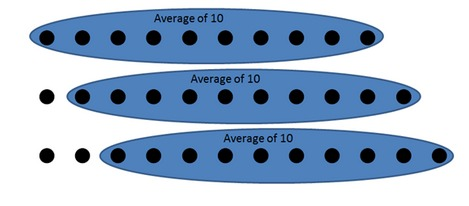
\includegraphics[height=6cm,width=90mm]{pics/movingAverage.jpg}
	\caption{Graphical depiction of the moving average.}
\end{figure}

Through the use of Null-Zone, the rate of change of the hand, and Moving Average, we manage to achieve much more stable flight.  There is now a reduced amount of "drifting" where the drone unintentionally moves without our control.  The controls have also become much more fine-tuned due to the fact the signals are now much clearer to the drone after our filtering and smoothing algorithms.  

\section*{Communication with the AR Drone}

The drone receives information through its own built-in Wi-Fi access point, where software may send instructions to. Using Python, we created a network socket in order to communicate with the drone through this Wi-Fi access point. Connecting through UDP (User Datagram Protocol), we send the flight signal to the drone. We decided to utilize UDP rather than TCP (Transmission Control Protocol) due to its speed. While TCP makes sure that all of the data that has been sent has definitely been received, this is not very important to us since our program sends 300 instructions to the AR Drone every second, and since human hands tend not to vary greatly within such a small time frame, it is not beneficial to make sure that every single instruction is received correctly. Since the security and hand-shaking process of TCP is unimportant to us, we decided to utilize UDP and minimize transmission delays which might hinder the pilot's control of the drone. As a measure to prevent loss of control over the Drone, we included a safeguard that commands the Drone to automatically land and shut down if no recognizable instructions have been received for 300 milliseconds. We put drone instructions inside of a callback method, which makes the program send instructions every time a frame is captured by the Leap Motion Controller. The controller captures 300 frames per second, or one frame approximately every 3.33 milliseconds, meaning that instructions are also sent to the drone every 3.33 milliseconds. If no instructions have been received for approximately 100 frames, or 300 milliseconds, it is evident that disconnection is strictly due to network problems.


\section*{Results}

The overall aim of this project was to create a simple interface for mapping intuitive hand gestures to the flight patterns of the AR Drone. We sought to do this by analyzing the position data that the Leap Motion generated by observing hand movements. In specific, we wanted to monitor the variation in degree from the mean position of the hand, which is when the user has his palm facing towards the floor and positioned directly over the Leap Motion. Our initial histograms showed us a distribution of data which seemed to match the normal distribution, so we decided to verify that assumption. We ran through the Shapiro-Wilks and found the previously mentioned General Extreme Value distributions were the best match for our data sets.

\begin{figure}[H]
	\centering
	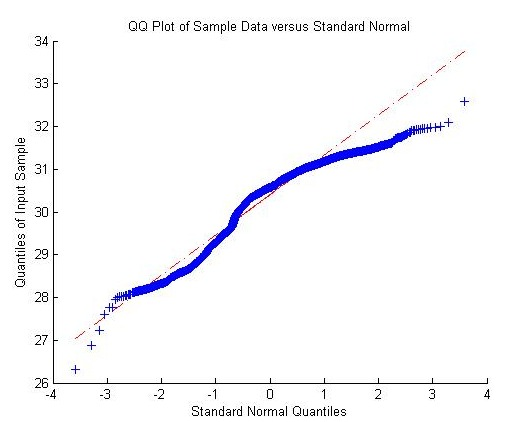
\includegraphics[height=6cm,width=90mm]{pics/qqLeft.jpg}
	\caption{QQ Plot for the Move Left gesture.}
\end{figure}

These tests provided us with a standard deviation for each position, which we then used to define the states for the hand. For example, when we moved into the "turn right" state, we found that the standard deviation from the mean of 45o was 1.8176 degrees. Using our proposed rule of including all data within two standard deviations of the mean as part of the state, we decided that the user's hand could vary by 3.6352 degrees in the counterclockwise or clockwise direction from the mean position. Similarly, we used the standard deviations to define regions within which the system would recognize that the hand was in a particular state.

The combination of the defined states and the flight-stabilizing algorithm resulted in precise control of the AR Drone. We tested each of the six states (both positive and negative orientations for yaw, pitch, and roll), and the Drone responded to each gesture with ease. We also tried slightly more complicated movements, such as navigating a figure-eight. While this proved to be more difficult than movement in general directions, we were still able to complete the flight path with less difficulty than with the default mobile interface. Based on the responsiveness of the Drone and the analysis of our data, we believe that we have achieved our objective of creating an intuitive, gesture-driven interface for the AR Drone.

\section*{Future Work}

There are several different improvements that can be made to the project. First, the transitions between the different states of movement can be improved. In our tests, we found that the Drone would not respond instantaneously to a change in the hand movement. This delay could be due to the time that the Leap Motion takes to detect and register hand movements through the frames, or it could be due to a definition of hand states that was not as precise. Regardless, the response of the Drone to quick changes in directions is an area for further work.
	
In addition to response time, the precision of control over the Drone should be worked on. In our figure-eight test, we found that the maneuvers did not provide enough control to navigate the path. Control was especially difficult when traversing the sharp turns. Our current system did not account for extremely precise movements of the Drone, and we feel that this is definitely an area for future work.
	
Finally, integrating the project with Google Glass and utilizing the Drone's video camera is the most interesting avenue for development. The goal would be to have the user stream video from the Drone's camera into the Google Glass and then manipulate the Drone based on the video feed. The Leap Motion would also be worn by the user so that he is not completely bound to one location by a laptop. This opens up exciting new possibilities for control, and the Drone could be developed to perform certain tasks, such as picking up objects in places that the user cannot reach. Although this is an ambitious plan, there could be immense rewards.


\section*{Contribution Breakdown}

\begin{center}
	\begin{tabular}{|c|c|c|c|c|}
		\hline
			 & Tae-Min & Felix & Nikhil & Shu \\
			 & Kim	   & Yeung & Shenoy & Xu \\
		\hline
			Report & 25\% & 25\% & 25\% & 25\% \\
		\hline
			Stability Testing & & 50\% & 50\% & & 
		\hline
			Stability Implementation & 50\% & & & 50\% \\
		\hline
			Drone Instructions & & 50\% & 50\% & & 
		\hline
			Leap Motion & 50\% & & & 50\% \\
		\hline
			Leap/Drone Integration & 25\% & 25\% & 25\% & 25\% \\
		\hline
	\end{tabular}
\end{center}

\begin{thebibliography}{1}

	\bibitem{cit1} Razali, Nornadiah Mohd, and Yap Bee Wah. "Power Comparisons of Shapiro-Wilks, Kolmogorov-Smirnov, Lilliefors, and Anderson-Darling Test." {\em Journal of Statistical Modeling and Analytics} 21-33 2.1 (2011): 21-33. Print.
		
	\bibitem{cit2} Shapiro, S.S.; Wilk, M.B. (1965). "An analysis of variance test for normality (complete samples)". {\em Biometrika} \textbf{52} (3-4):  591-611. doi:10.1093/biomet/52.3-4.591. JSTOR 2333709. MR 205384. p. 593.

	\bibitem{cit3} Hazewinkel, Michael, ed. (2001), "Normal distribution", {\em Encyclopedia of Mathematics}, Springer, ISBN 978-1-55608-010-4

	\bibitem{cit4} Scott, David. "Quantile-Quantile (q-q) Plots." {\em Online Statistics Education: A Free Resource for Introductory Statistics}. National Science Foundation's Division of Undergraduate Eduation, n.d. Web. 03 May 2014.

	\bibitem{cit5} David, Lane M. "Histograms." {\em Histograms}. National Science Foundation's Division of Undergraduate Education, n.d. Web. 01 May 2014.

	\bibitem{cit6} Arshad M., Rasool, M.T. And Ahmad, M.I. (2003). {\em Anderson Darling and Modified Anderson Darling Tests for Generalied Pareto Distribution}. Pakistan journal of Applied Sciences 3(2),pp.85-88.

	\bibitem{cit7} Lilliefors, H.W. (1967). {\em On the Kolmogorov-Smirnov Test for Normality with Mean and Variance Unknown}. Journal of American Statistical Association, Vol. 62, No. 18, pp. 399-402

	\bibitem{cit8} Conover, W.J. (1999). {\em Practical Nonparametric Statistics}. Third Edition, John Wiley and Sons, Inc. New York. pp. 428-443 (6.1)
	
	\bibitem{cit9} "Frame." {\em Frame - Leap Motion Python SDK V1.2 Documentation.} Leap Motion, n.d. Web. 20 May 2014
		
	\bibitem{cit10} "Cramer-von Mises criterion." {\em Wikipedia: the Free Encyclopedia.} N.p., n.d. Web. 20 May 2014. http://en.wikipedia.org/wiki/Cram\%C3\%A9r\%E2\%80\%93von\_Mises

	\bibitem{cit11} "Getting Frame Data." www.developer.leapmotion.com. Leap Motion, n.d. Web. 20 May 2014
\end{thebibliography}



\end{document}
